Ein Beispiel für Code:
\lstinputlisting[language=JAVA]{Code/REST-Interface/src/PackageIdModelEndpoint.java}
Ein Beispiel für das Einfügen einer Grafik:
\begin{figure}[H]
\centering
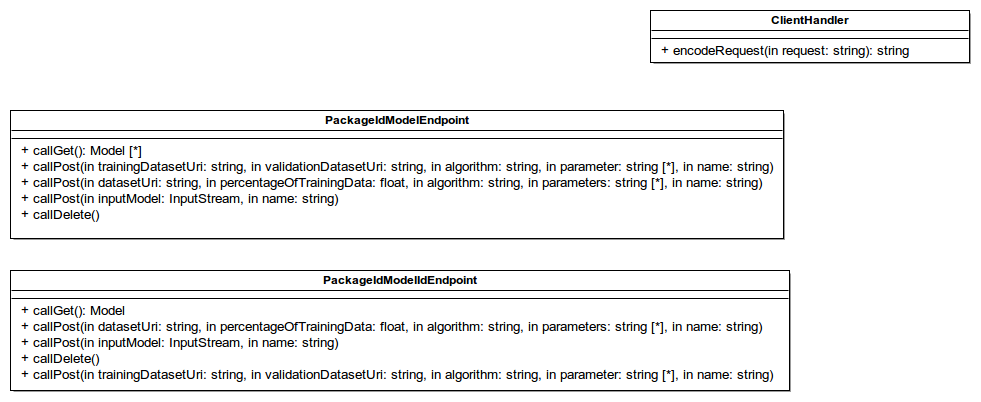
\includegraphics[width=0.7\linewidth]{Grafik/Diagramme/Restschnittstelle}
\caption[Test-Klassendiagramm]{Klassendiagramm für Test}
\label{fig:REST-Interface}
\end{figure}
Und noch einmal:
\lstinputlisting[language=JAVA]{Code/REST-Interface/src/PackageIdModelIdEndpoint.java}